\styledchapter[Stappen in een machine learning pipeline]{stappen-in-een-machine-learning-pipeline}

Een ML pipeline is zoals beknopt beschreven in \autoref{subsec:opzetten-pipeline} een collectie van stappen dat wordt doorlopen om een model te trainen. Elke stap bevat een aantal acties dat wordt uitgevoerd, zoals onbruikbare data weghalen of de prestatie analyseren. De stappen en acties worden in \autoref{sec:de-stappen-in-een-machine-learning-pipeline} uitgelegd. Een van de stappen in een pipeline is het trainen van het model. Om een idee te krijgen van ML en modellen trainen wordt dit kort uitgelegd.

\section{Wat is machine learning?}\label{sec:wat-is-machine-learning}
ML houdt in dat een computer een taak kan uitvoeren zonder ervoor expliciet geprogrammeerd te zijn. Dit wordt gedaan door een ML model te laten leren van een gegeven dataset. Vervolgens kan er een voorspelling worden gemaakt \cite[p.~1-3]{introduction-to-machine-learning}.

De domeinen deep learning (DL), neural networks (NN) en artificial intelligence (AI) komen vaak voor als het over ML gaat. Zoals weergegeven in \autoref{fig:ai-ml-nn-dl} is te zien dat ML een subset is van AI, NN een subset van ML en als laatste DL dat een subset is van NN.

Bij AI wordt niet alleen ML toegepast, maar ook concepten zoals beredeneren, plannen, vooruitdenken, onthouden en terug refereren. Een voorbeeld hiervan is dat een ML model kan voorspellen wat het volgende woord in een zin kan zijn, maar een AI kan beredeneren waarom de zin gebouwd is zoals het is en hoe het binnen de context van de alinea past \cite{ml-think-about-ml-brownlee}.

\begin{figure}[hbt!]
  \centering
  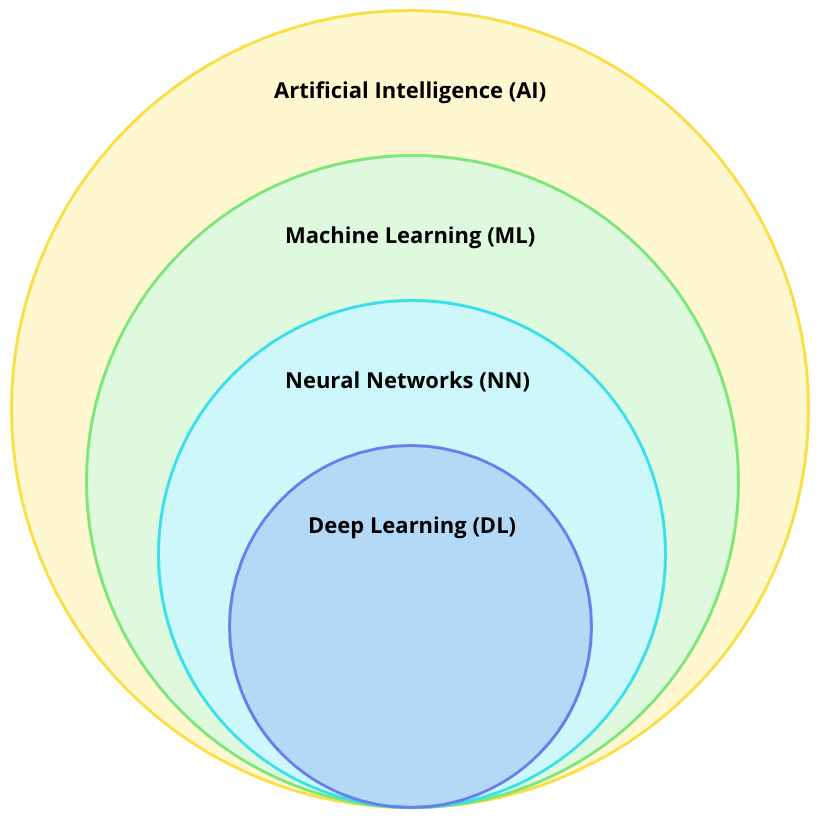
\includegraphics[width=0.48\textwidth]{chapter-4/AI-ML-NN-DL.png}
  \caption{Machine learning in de context van andere domeinen}
  \label{fig:ai-ml-nn-dl}
\end{figure}

Een NN bestaat uit een collectie van nodes dat gemodelleerd is naar de hersenen. Een NN heeft minimaal 3 lagen: een input laag, een verborgen laag en een output laag. Elke laag bevat neuronen dat data als input kan krijgen en data als output aan de volgende laag meegeeft. DL is een NN dat meerdere verborgen lagen bevat \cite{ml-neural-network-nicholson}.

In het ML domein bestaan talloze algoritmes om voorspellingen te maken. In de [BIJLAGE LINK] is een mind-map te vinden van de algoritmes die gedurende de scriptie naar voren zijn gekomen. Het grotendeels kan gegroepeerd worden in vier stijlen: supervised, unsupervised, semi-supervised en reinforcement learning. In de [BIJLAGE LINK] is meer informatie over de stijlen te vinden.

Het trainen van een model is een proces waarbij vooraf data wordt opgeschoond en achteraf de prestatie van het model wordt gevalideerd. Normaliter wordt dit gedaan door specifieke code te schrijven voor deze taken. Een valkuil is dat de code niet bij elke developer werkt en schaalt niet in alle gevallen naar een productie omgeving. Een manier om dit wel te behalen is om te werken met ML pipelines. Zoals kort uitgelegd in \autoref{subsec:opzetten-pipeline} bestaat een ML pipeline uit stappen en acties. Er is echter geen consensus binnen het ML domein over wat de juiste stappen en acties in een pipeline zijn. Voor de scriptie is gekozen voor een pipeline van Hapke en Nelson uit het boek "Building Machine Learning Pipelines". Het boek is gemaakt en gepubliceerd door O'Reilly; een bekend en gecrediteerd bedrijf dat boeken maakt binnen het software engineering domein.

\section{De stappen in een machine learning pipeline}\label{sec:de-stappen-in-een-machine-learning-pipeline}
Een ML pipeline begint met het opnemen van data en eindigt met het ontvangen van feedback om de prestatie van het model te verbeteren. De pipeline bevat een aantal stappen zoals data voorbereiden, het model trainen en het uitrollen van het model (\autoref{fig:model-lifecycle-oreilly}).

\begin{figure}[hbt!]
  \centering
  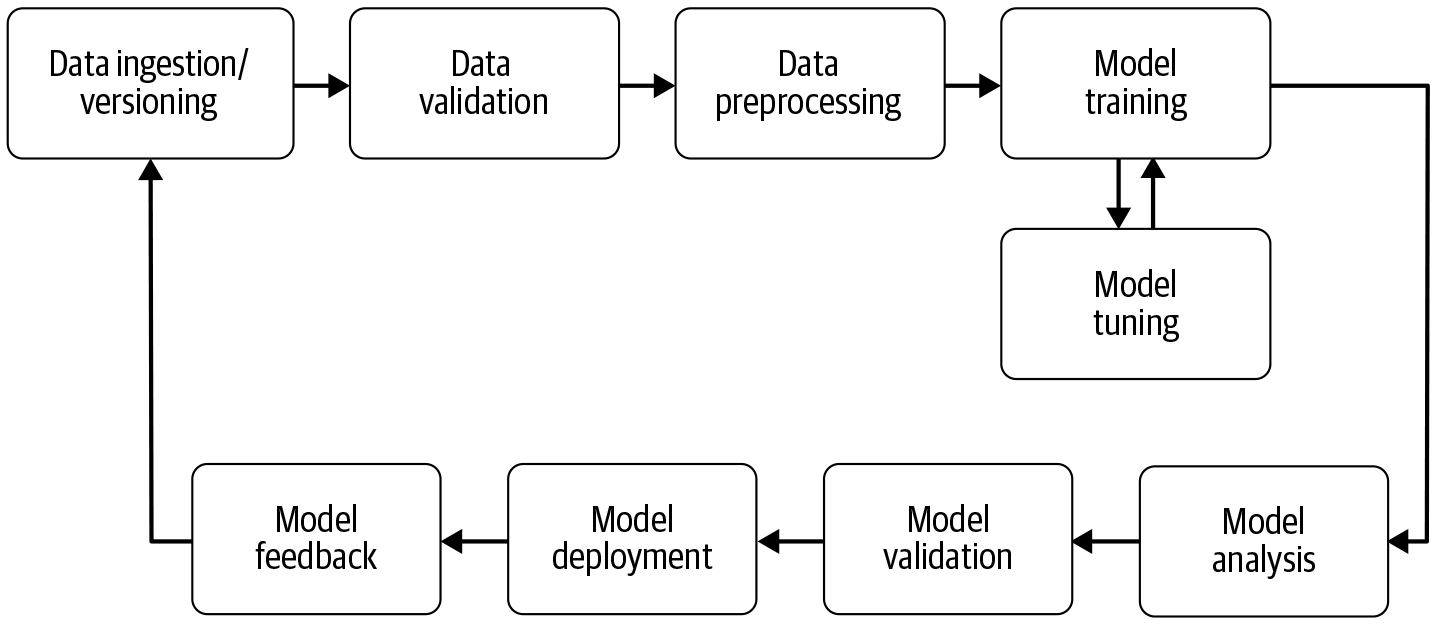
\includegraphics[width=.8\textwidth]{chapter-4/ml-pipeline-lifecycle-oreilly.png}
  \caption{Lifecycle van een model volgens Hapke en Nelson \cite[p.~4]{building-machine-learning-pipelines-oreilly}.}
  \label{fig:model-lifecycle-oreilly}
\end{figure}

In totaal zijn er, zonder de feedback loop stap, acht stappen dat elke keer doorlopen moeten worden om een model te trainen. In de volgende subkoppen zullen de stappen worden doorlopen met een korte uitleg over wat er gebeurd in een stap. 

\subsection{Stap 1: Data opname en versiebeheer (Data ingestion/versioning)}\label{subsec:data-opname-en-versiebeheer}
De eerste stap in de pipeline is het opnemen van data. Met deze data zal het model getraind, gevalideerd en getest worden. De dataset kan van een of meerdere bronnen komen, zoals lokaal, een online opslag locatie of van een database. Zodra de data is ingeladen, moet het verdeeld worden tussen een train, validatie en test dataset. Normaal gebeurt dit met een split ratio van 6:2:2. De train dataset is 60\% en de validatie en test datasets zijn allebei 20\% van de originele dataset \cite[p.~27-37]{building-machine-learning-pipelines-oreilly}.

Een use case van een pipeline is dat een nieuw model getraind kan worden door een geüpdatet dataset te gebruiken. Dit wordt gedaan door de voorgaande dataset te gebruiken waarbij nieuwe data is toegevoegd. Door het gebruik van verschillende datasets is het verstandig om versiebeheer toe te passen. Zo is goed te zien welk dataset welk model produceert. Een versie geven aan een dataset gebeurt voordat de dataset wordt ingeladen \cite[p.~39-40]{building-machine-learning-pipelines-oreilly}. Versiebeheer voor datasets kan bijvoorbeeld met DVC \cite{dvc} of Pachyderm \cite{pachyderm}.

% De iris dataset wordt in \autoref{fig:step-1} geïmporteerd door middel van code. Normaal gesproken zou, voordat deze code uitgevoerd wordt, een versie gegeven worden aan de dataset. Omdat de schaal van dit voorbeeld klein is en om de voorbeeld reproduceerbaar te houden is dit niet gedaan. De dataset wordt aangemaakt met de namen voor de kolommen op regel 5 net zoals het voorbeeld in \autoref{table:example-iris-dataset}. Vervolgens is de dataset onder de variabel naam \(dataset\) beschikbaar voor de komende stappen.

% \begin{figure}[hbt!]
%   \centering
%   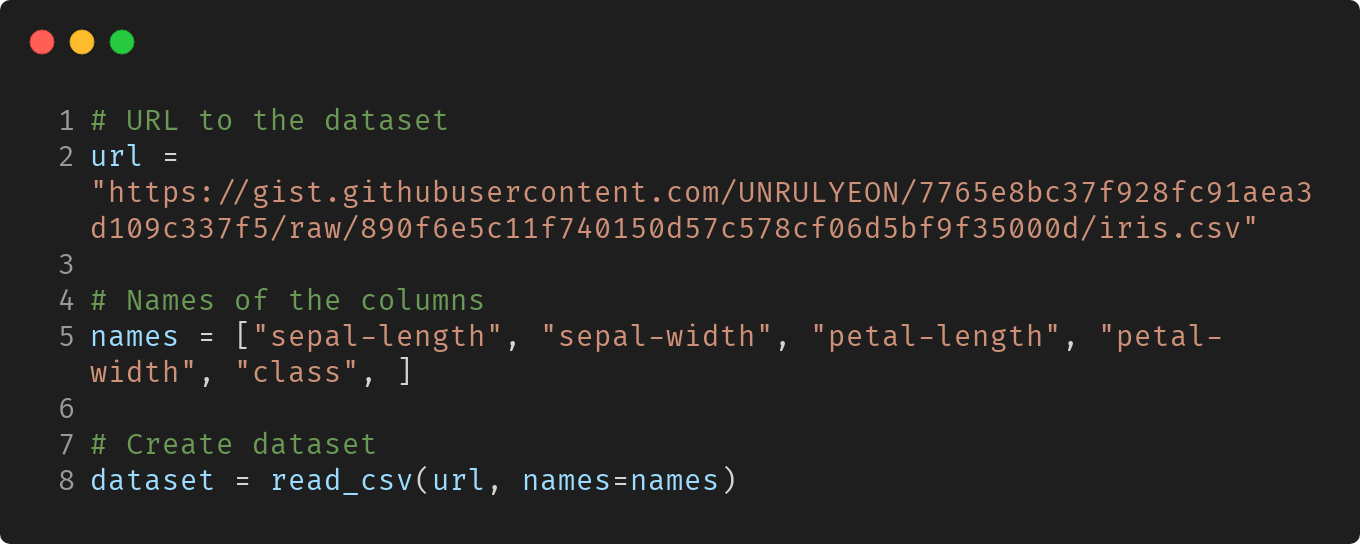
\includegraphics[width=.8\textwidth]{chapter-4/step-1.png}
%   \caption{Dataset importeren}
%   \label{fig:step-1}
% \end{figure}

\subsection{Stap 2: Data validatie (Data validation)}\label{subsec:data-validatie}
Nu de dataset verdeeld is, een versie heeft en op een bereikbare plek is, kan de data gevalideerd worden. Deze stap is vooral belangrijk om te voorkomen dat een model wordt getraind dat niet nuttig is aangezien het trainen veel tijd in beslag kan nemen. Een bekende uitdrukking is "garbage in = garbage out". Dit betekent dat als de dataset niet goed is, het model ook niet goed zal presteren \cite[p.~43]{building-machine-learning-pipelines-oreilly}. Tijdens de validatie stap wordt gecontroleerd op het volgende:

\begin{itemize}
  \item Afwijkingen in de dataset
  \item Wijzigingen in de structuur
  \item Algemene statistieken in vergelijkingen met voorgaand datasets \cite[p.~44]{building-machine-learning-pipelines-oreilly}
\end{itemize}

Bij het controleren van afwijkingen in de dataset wordt gekeken naar waardes die opmerkelijk zijn. Afwijkende waardes liggen te ver van het gemiddelde en kan een verkeerd beeld schetsen bij het trainen van het model. Deze uitschieters kunnen simpelweg uit de dataset gefilterd worden.

Het kan voorkomen dat bij een nieuw dataset de type van waardes zijn gewijzigd. Een \(int\) kan bijvoorbeeld veranderd zijn in een \(string\) of \(boolean\). Er is dan sprake van een wijziging in de structuur van de dataset. Dit is problematisch omdat er een vertaalstap gemaakt moet worden naar iets bruikbaars. Als dit niet mogelijk is moeten de waardes uitgefilterd worden wat de prestatie van het model negatief kan beïnvloeden.

De algemene statistieken is een hulpmiddel om te controleren op afwijkingen en wijzigingen. Vaak kan de controle in een oogopslag gedaan worden. 

% De code voor het genereren van de statistieken hangt af van hoe de dataset eruit ziet en wat er gegenereerd moet worden. In \autoref{fig:step-2} is te zien hoe statistieken worden gegenereerd uit de iris dataset.

% \begin{figure}[hbt!]
%   \centering
%   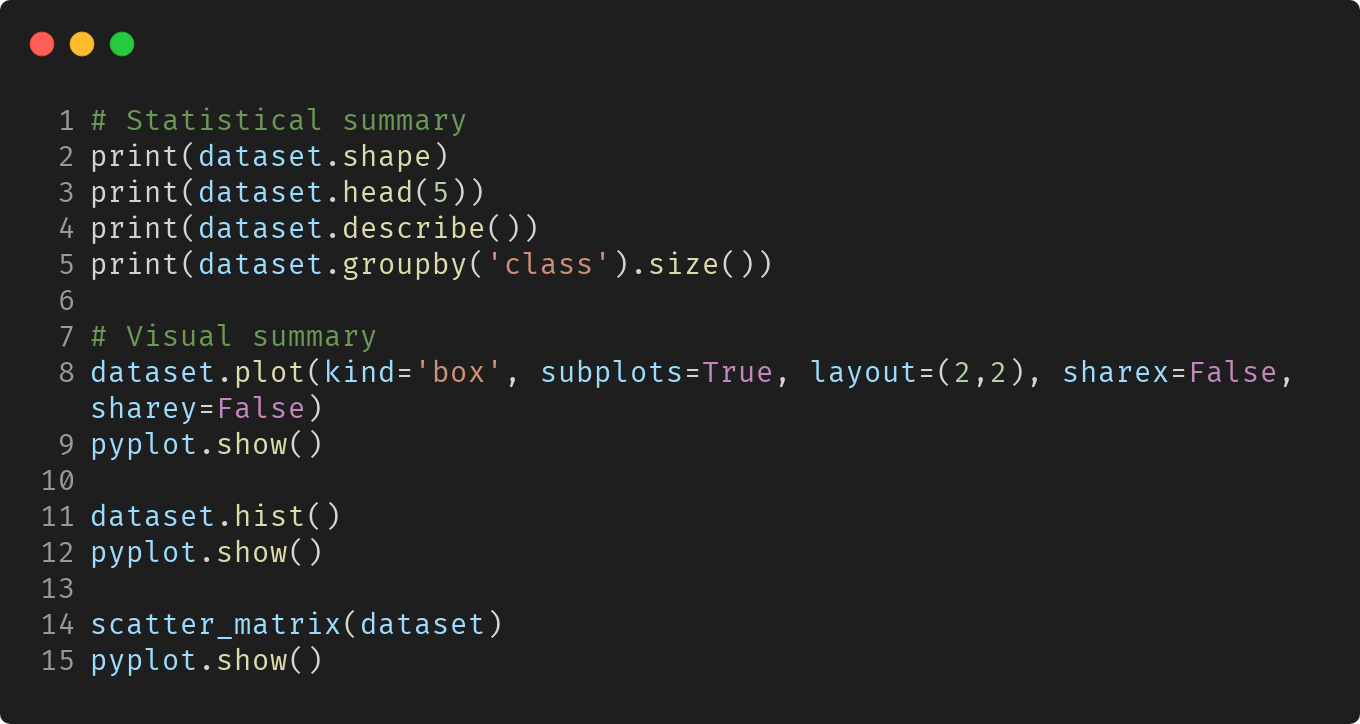
\includegraphics[width=.8\textwidth]{chapter-4/step-2.png}
%   \caption{Statistieken genereren}
%   \label{fig:step-2}
% \end{figure}

% \begin{figure}[hbt!]
%   \centering
%   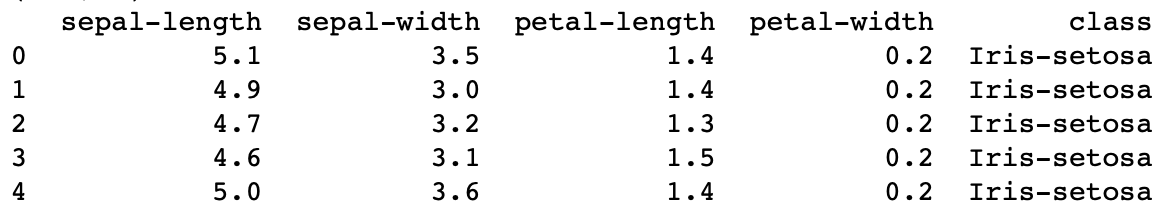
\includegraphics[width=.9\textwidth]{chapter-4/step-2-head-dataset.png}
%   \caption{Statistieken - Eerste 5 regels van de iris dataset}
%   \label{fig:step-2-head-dataset}
% \end{figure}

% \begin{figure}[hbt!]
%   \centering
%   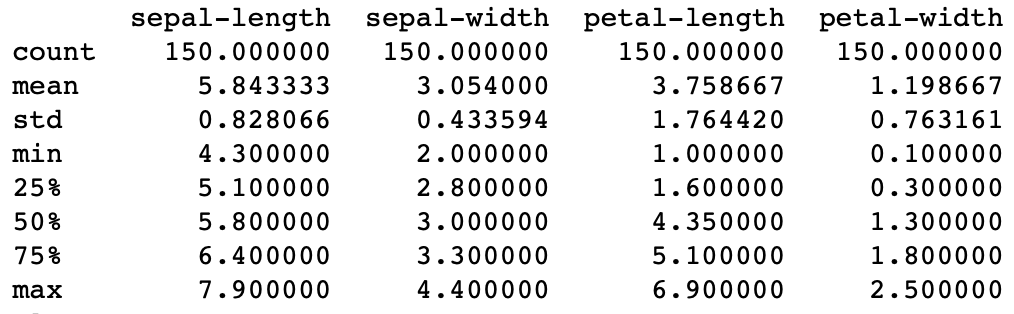
\includegraphics[width=.8\textwidth]{chapter-4/step-2-dataset-described.png}
%   \caption{Statistieken - De iris dataset beschreven}
%   \label{fig:step-2-dataset-described}
% \end{figure}

% \begin{figure}[hbt!]
%   \centering
%   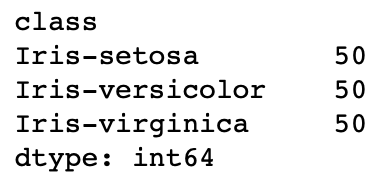
\includegraphics[width=.4\textwidth]{chapter-4/step-2-grouped-by-class.png}
%   \caption{Statistieken - Iris dataset gegroepeerd}
%   \label{fig:step-2-grouped-by-class}
% \end{figure}

\subsection{Stap 3: Data voorbereiden (Data preprocessing)}\label{subsec:data-voorbereiden}
Het voorbereiden van de dataset is een stap dat de prestatie van het model verbetert en het proces van het trainen versneld. Deze stap kan verdeeld worden in twee sub-stappen: het opschonen en het optimaliseren van de dataset.

Bij het opschonen worden bijvoorbeeld duplicaten of waardes die onbruikbaar zijn uit de dataset weggehaald. Onbruikbare waardes zijn waardes die simpelweg niet kloppen of verkeerd zijn ingevoerd. Hierbij kan bijvoorbeeld gedacht worden aan een medewerken die de interactietijd met een klant moet bijhouden, maar is vergeten om de eindtijd te noteren. Voor het algoritme zal het dan lijken alsof de medewerker een klant tot sluitingstijd heeft geholpen.

Datasets kunnen geoptimaliseerd worden om twee redenen: algoritmes werken sneller met waardes die dichter bij \(0\) liggen en algoritmes kunnen niet met elke waarde in de dataset omgaan. Om de efficiëntie van het algoritme te verbeteren kunnen een aantal technieken gebruikt worden:

\begin{itemize}
  \item Schalen
  \item[] Bij het schalen van data worden de waardes getransformeerd waardes dat ligt tussen een schaal, zoals tussen \(0\) en \(100\) of \(0\) en \(1\). Bij het schalen wordt het \textbf{bereik} getransformeerd \cite{scale-and-normalize-data}. 
  \item Normaliseren
  \item[] Als een dataset wordt gestandaardiseerd, worden de waarden getransformeerd in een standaard normale verdeling waarbij het gemiddelde \(0\) en de afwijking \(1\) is. Hierbij wordt de \textbf{vorm} van de dataset getransformeerd \cite{scale-and-normalize-data}. Het normaliseren is belangrijk als het algoritme waardes vergelijkt met verschillende eenheden \cite{feature-scaling-standardization}. In sommige gevallen is normalisering een vereiste bij een aantal algoritmes \cite{data-transformation-standardization-vs-normalization}.
  \item Categorisch codering
  \item[] Een groot aantal algoritmes kan alleen omgaan met numerieke waardes. Het kan voorkomen data datasets categorische waardes bevatten. Dit zijn waardes dat een label voorstellen, zoals \(first\), \(second\) of \(third\). Om deze waardes te gebruiken moeten ze worden gecodeerd als een numerieke waarde. De label kan als de waarde \(1\) of \(2\) gecodeerd worden. Deze techniek heet integer encoding en kan gebruikt worden als de volgorde van de codering klopt. Een andere techniek om waardes te coderen heet hot encoding. Deze techniek wordt gebruikt waarbij de labels geen relatie met elkaar hebben en maakt gebruik van meerdere waardes om een label te beschrijven:
  \begin{center}
    $$\begin{bmatrix}
      \textbf{Animal} & \textbf{C1} & \textbf{C2} & \textbf{C3}\\
      cat & 1 & 0 & 0 \\
      dog & 0 & 1 & 0 \\
      mouse & 0 & 0 & 1 \\
    \end{bmatrix}$$
  \end{center}


\end{itemize}

Dit is een goed moment om het getransformeerde dataset op te slaan als "tussen-dataset"\space zodat deze stap niet herhaalt hoeft te worden. Het voorbereiden van grote datasets kan een grote hoeveelheid tijd in beslag nemen.

\subsection{Stap 4 en 5: Model trainen en tunen (Model training and Model tuning)}\label{subsec:model-trainen-en-tunen}
Na het valideren en voorbereiden van de dataset kan het model getraind worden. Het trainen gaat door middel van een ML algoritme. Een algoritme is vergelijkbaar met een conventionele algoritme in software engineering zoals bijvoorbeeld binary search, merge sort en depth first search. Het algoritme slaat na het trainen met de dataset regels, nummers en algoritme specifieke data structuren op in de vorm van een model. Het algoritme kan worden gezien als een specifiek programma waarmee, gegeven een input, voorspellingen mee gedaan kan worden \cite{ml-algorithm-model-difference}.

Elk algoritme heeft variabelen om er voor te zorgen dat het algoritme beter aansluit op de dataset. Deze variabelen heten \textit{hyperparameters}. Het algoritme heeft standaard hyperparameters die niet altijd de optimale prestatie behalen. Op een heuristische wijze kunnen de optimale hyperparameters gevonden worden \cite{ml-model-hyper-parameter-brownlee}. Dit proces heet \textit{tunen}.

In \autoref{fig:hyperparameter-example-0.1} en \autoref{fig:hyperparameter-example-100} is te zien hoe de \(gamma\) hyperparameter van een SVC algoritme invloed heeft op het model. Dit algoritme classificeert op basis van gegeven waardes. De waardes worden geplot en zal binnen een van de drie kleuren vallen. Het model met als hyperparameter waarde \(100\) zal vaker de classificatie met de bruine kleur als voorspelling geven dan als de waarde \(0.1\) zou zijn.

\begin{figure}[hbt!]
  \centering
  \begin{minipage}{0.45\textwidth}
      \centering
      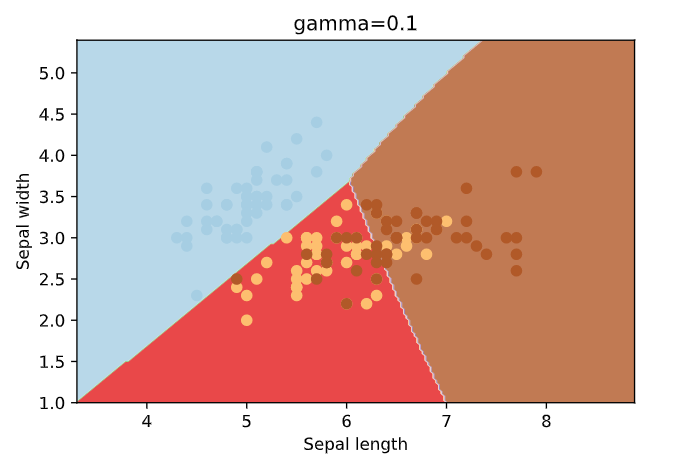
\includegraphics[width=1\textwidth]{./chapter-4/hyperparameter-0.1.png}
      \caption{Gamma hyperparameter van een SVC algoritme met waarde 0.1}
      \label{fig:hyperparameter-example-0.1}
  \end{minipage}\hfill
  \begin{minipage}{0.45\textwidth}
      \centering
      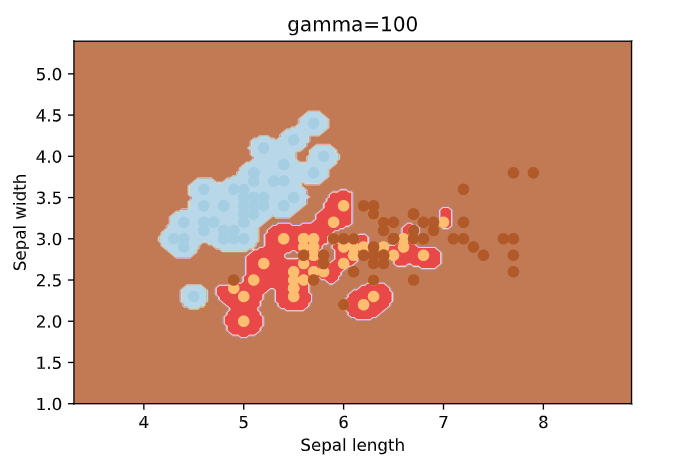
\includegraphics[width=1\textwidth]{./chapter-4/hyperparameter-100.png}
      \caption{Gamma hyperparameter van een SVG algoritme met waarde 100}
      \label{fig:hyperparameter-example-100}
  \end{minipage}
\end{figure}

\subsection{Stap 6 en 7: Model analyse en validatie (Model analysis and Model validation)}\label{subsec:model-analyse-en-validatie}
Na het trainen en tunen kan analyse en validatie plaats vinden. Bij het analyseren wordt de prestatie van het model vergeleken met voorgaande modellen. Om dit te doen kan, net als in \autoref{subsec:data-validatie}, statistieken gegenereerd worden van het model. De soort statistiek hangt af van wat voor soort algoritme is gebruikt. Een classificatie algoritme heeft bijvoorbeeld andere statistieken dan een regressie algoritme. Op basis van de uitkomst kan de dataset of hyperparameters aangepast worden om de accuraatheid te verhogen.

Met de validatie van een model moet er gekeken worden met een genuanceerd perspectief. Validatie gaat namelijk over hoe eerlijk een model is als er gekeken wordt naar een bepaalde groep. Een groep kan gedefinieerd worden als geslacht, etniciteit, locatie of leeftijd. Het kan namelijk voorkomen dat de dataset voornamelijk bestaat uit bijvoorbeeld vrouwen. Dit \textit{kan} ervoor zorgen dat het model minder accurate voorspellingen maakt voor mannen \cite[p.~109-110]{introduction-to-machine-learning}. Een voorbeeld waar het gebruik van ML grote negatieve gevolgen had was de toeslagenaffaire in 2020. De Nederlandse overheid maakte gebruik van een systeem dat aangaf of een burger mogelijk bijstandsfraude had gepleegd. Het systeem maakte gebruikt van ML om fraude aan te geven. Jaren na het gebruik bleek dat er sprake was van etnische profilering. De dataset bestond voornamelijk uit immigranten uit Islamitische landen. Het systeem heeft hierdoor een \textit{bias} \cite{ml-fairness-dutch-syri}.

\subsection{Stap 8: Model uitrollen (Model deployment)}\label{subsec:model-uitrollen}
Na het analyseren en valideren kan het model uitgerold worden. Het uitrollen kan op twee manieren: inbakken in een app of serveren met een \acrfull{api}.

Met het inbakken in een app wordt bedoelt dat het model meegenomen wordt als de app gebouwd wordt. Voordelen van deze methode is dat het model offline bruikbaar is en de rekenkracht van het apparaat gebruikt kan worden om te voorspellen of classificeren. Een nadeel is dat het model niet makkelijk geüpdatet kan worden.

Een model serveren door middel van een \Acrshort{api}. De app dat het model wilt gebruiken zal een request moeten doen met input. De \Acrshort{api} geeft de input door aan het model. Het model geeft een predictie terug dat de \Acrshort{api} doorstuurt naar de applicatie. Het updaten van het model gaat gemakkelijker dan het model inbakken met een app. Een nadeel is de eis dat de app een internetverbinding moet hebben om het model te gebruiken \cite[p.~130]{introduction-to-machine-learning}.

In \autoref{fig:step-8-deploy-model} is te zien hoe een model geserveerd wordt via een \Acrshort{api}. Een endpoint genaamd \("classify"\) is gedefinieerd waarop een \(POST\) request gedaan kan worden. De endpoint haalt de input uit de request en geeft het door aan het model. De model maakt vervolgens een predictie dat uiteindelijk naar de app teruggestuurd wordt.

\begin{figure}[hbt!]
  \centering
  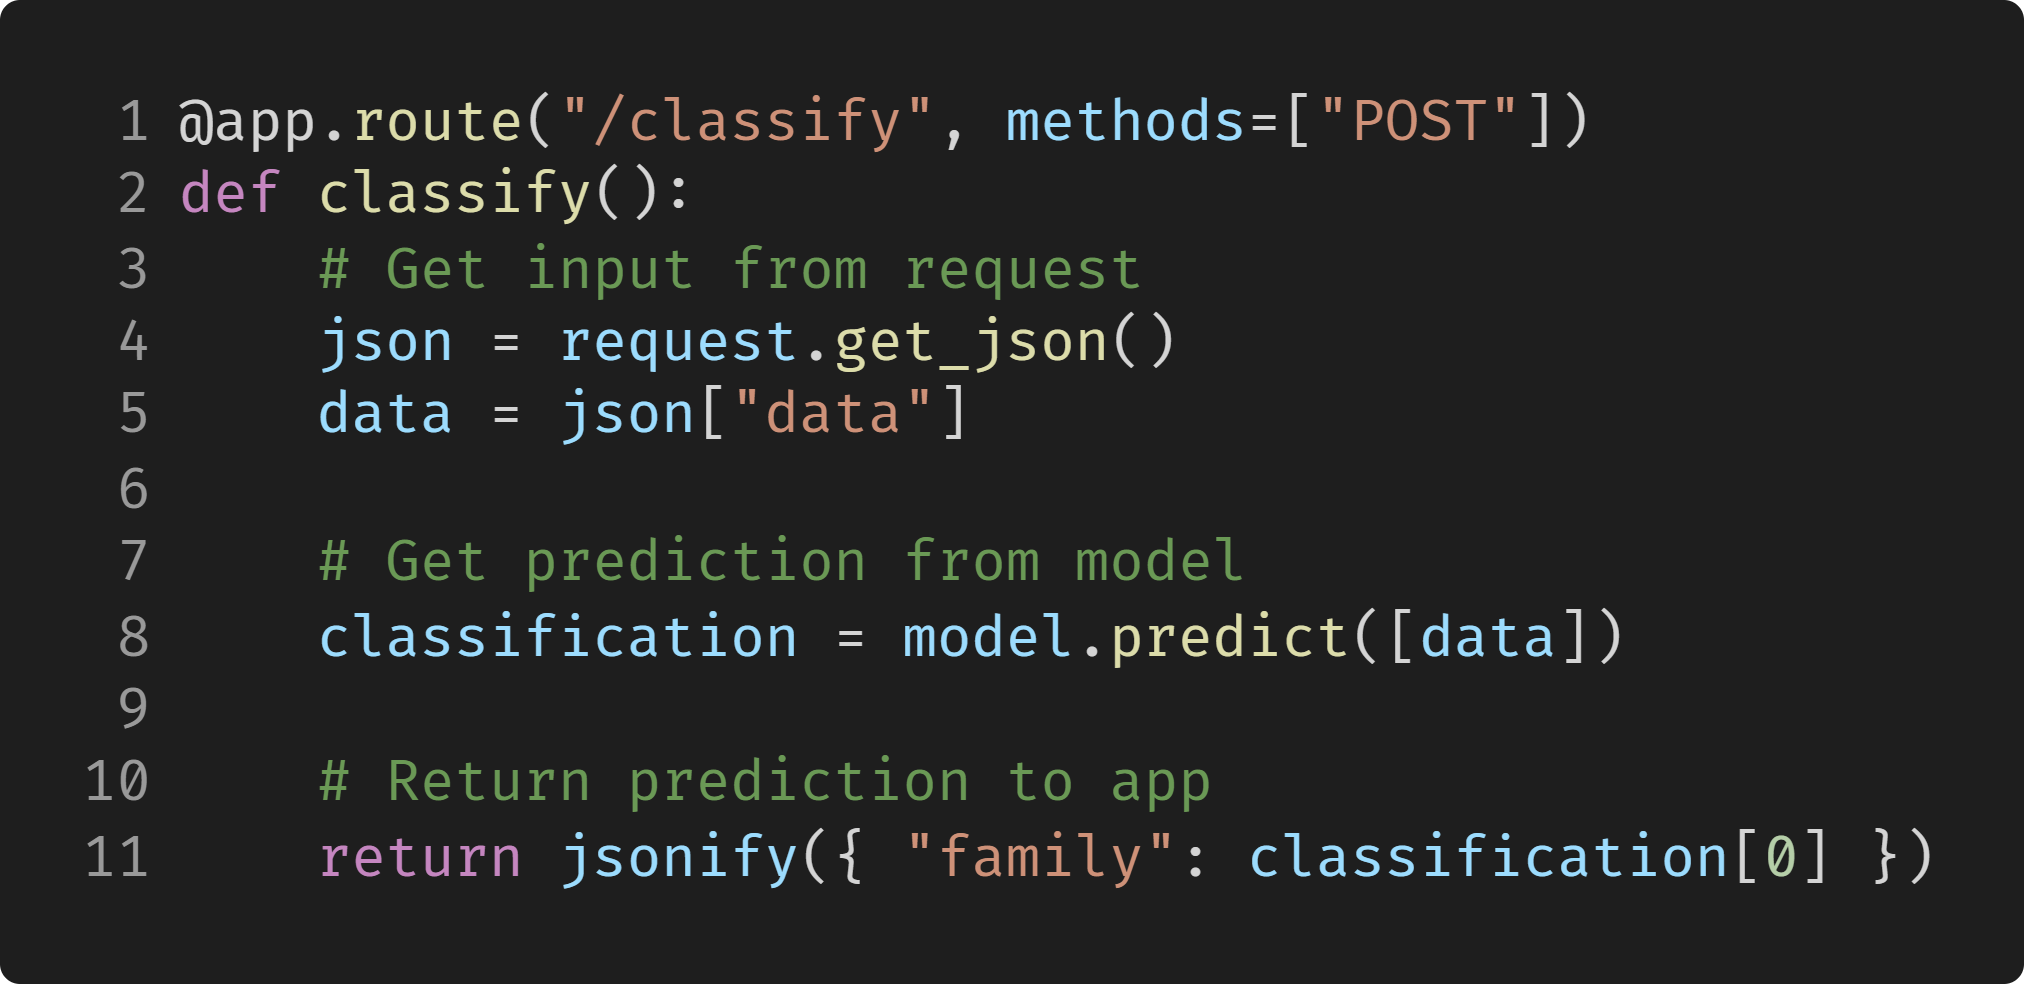
\includegraphics[width=.75\textwidth]{chapter-4/step-8-deploy-model.png}
  \caption{Model uitgerold met behulp van een \Acrshort{api}.}
  \label{fig:step-8-deploy-model}
\end{figure}

\subsection{Stap 9: Feedback loop (Model feedback)}\label{subsec:feebdack-loop}
Om het model continue te verbeteren kan feedback verzameld worden. De feedback geeft een beeld van de effectiviteit van het model in een productie omgeving. Feedback kan verdeeld worden in twee soorten: impliciet en expliciet \cite[p.~264]{introduction-to-machine-learning}.

Het verzamelen van impliciete feedback wordt gedaan zonder dat de gebruiker zich daar bewust van is. Dit wordt gedaan door bij te houden of een voorspelling geschikt is. Een voorbeeld van deze methode is het bijhouden of een gebruiker een video kijkt dat door het algoritme voorgesteld is.

In tegenstelling tot impliciet wordt bij expliciete feedback gevraagd aan de gebruiker of een voorspelling gepast is. Een voorbeeld van deze vorm in de praktijk is hoe YouTube expliciete feedback vraagt (\autoref{fig:step-9-explicit-feedback}). Naast het aangeven of de voorspelling gepast was, kan de gebruiker ook aangeven waarom de video gepast was.

\begin{figure}[hbt!]
  \centering
  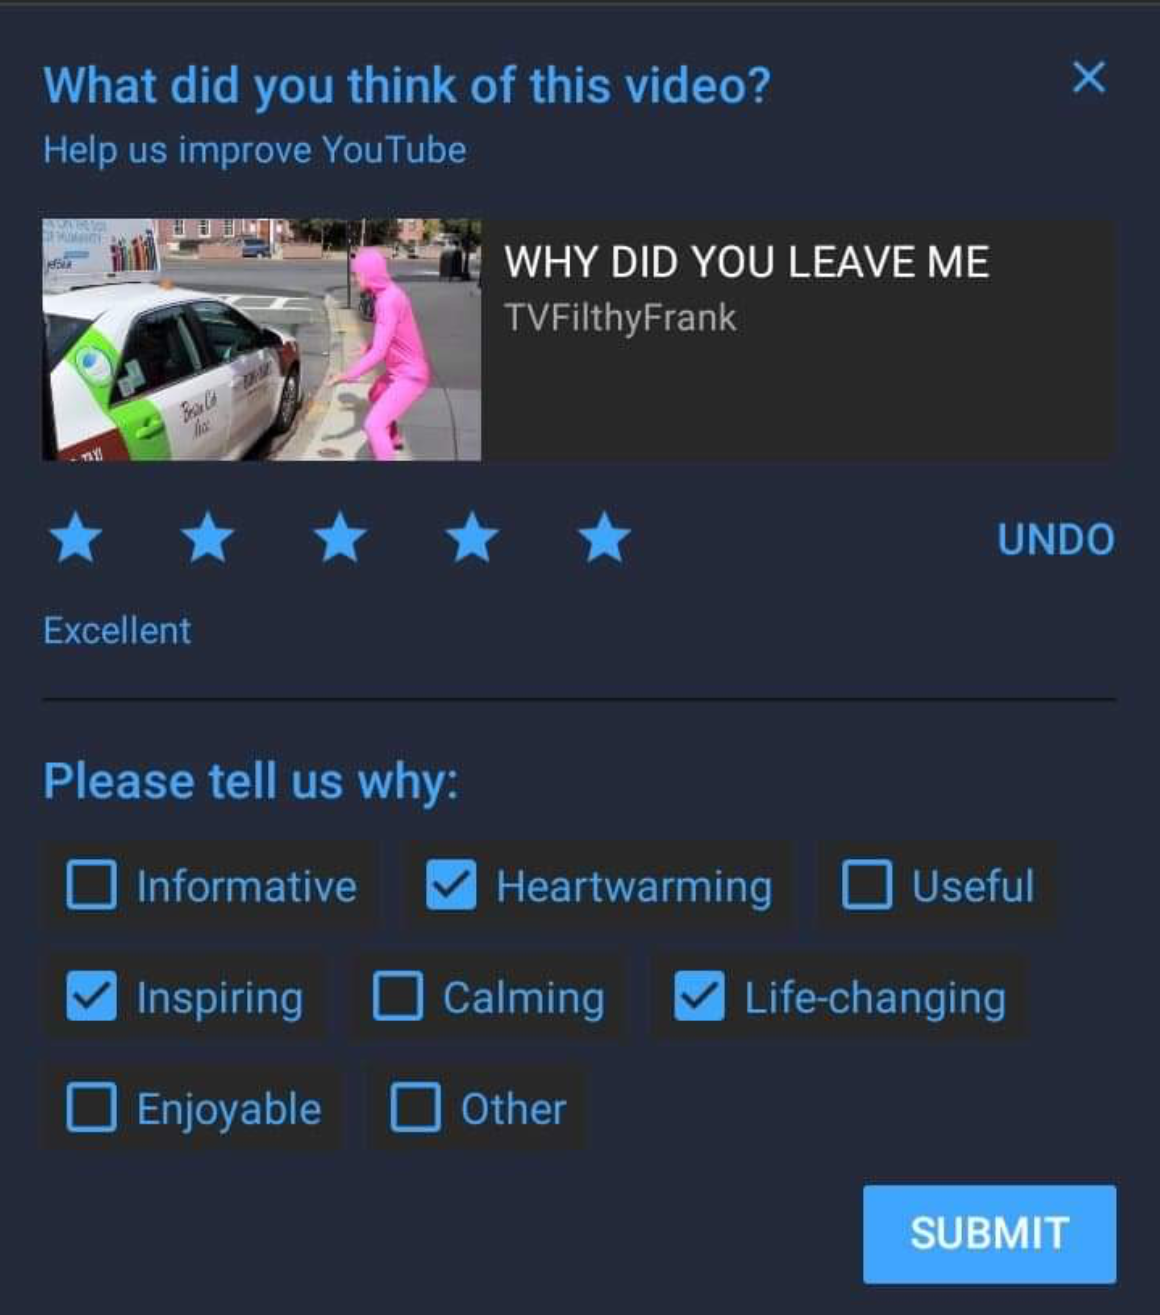
\includegraphics[width=.5\textwidth]{chapter-4/step-9-explicit-feedback.png}
  \caption{Vorm van expliciete feedback gebruikt door YouTube.}
  \label{fig:step-9-explicit-feedback}
\end{figure}

Het verzamelen van feedback is niet noodzakelijk maar helpt met het verbeteren van het model. Deze stap gaat samen met een nieuwe dataset naar de eerste stap in de lifecycle (\autoref{fig:model-lifecycle-oreilly}). Met de nieuwe dataset en de feedback kan een nieuw model getraind worden dat beter presteert dan de voorganger.

\section{Conclusie}\label{conclusie}
In dit hoofdstuk is er onderzoek gedaan naar de antwoord op de deelvraag: \textbf{D1: Waar bestaat een machine learning pipeline uit?} Het onderzoek is uitgevoerd met behulp van zowel digitale bronnen als een boek.

Een ML pipeline bestaat uit verschillende stappen die op hun beurt bestaan uit acties. De stappen zijn gericht op het waarborgen van de kwaliteit van de dataset en model, het voorbereiden van de dataset en het trainen van het model. Daarnaast kan het model uitgerold worden in een productie omgeving en kan er feedback verzameld worden over de prestatie van het model volgens gebruikers.

De acties in de stappen moeten bij het eerste gebruik van de pipeline gedefinieerd worden. De acties kan bijvoorbeeld het filteren van onbruikbare data, een model trainen of statistieken genereren zijn, Als dit vast staat, kan de pipeline hergebruikt worden om nieuwe modellen te trainen met nieuwe datasets. Op deze manier is een ML pipeline een gestructureerde en reproduceerbare proces.

\section{Advies}\label{advies}
Het in gebruik nemen van een ML pipeline werkwijze is initieel ingewikkeld maar lonend op lange termijn. Het opzetten van de pipeline en de acties definiëren kost tijd en kennis. Echter als dit eenmaal gedaan is, kan eenvoudig een verbeterd model worden getraind door een nieuwe dataset aan te leveren. Een verbeterd model is vrijwel gegarandeerd omdat stappen in de pipeline de dataset en het model analyseren en valideren.

\subsection{Machine learning pipeline verbeteringen}\label{subsec:machine-learning-pipeline-verbeteringen}
Zoals eerder aangegeven in \autoref{sec:wat-is-machine-learning} bestaat er niet één ML pipeline dat correct is. Een ML pipeline is een werkwijze waarbij de stappen anders geïnterpreteerd kan worden. Hierdoor is er geen regelmaat tussen verschillende pipelines. Dit is ook niet haalbaar aangezien stappen gemaakt kunnen worden dat specifiek is voor het algoritme of workflow van het bedrijf. De stappen in de pipeline van Hapke en Nelson (\autoref{fig:model-lifecycle-oreilly}) is een valide basis maar kan uitgebreid worden om de ervaring van developers te verbeteren. In stap 4 en 5 (\autoref{subsec:model-trainen-en-tunen}) wordt een model getraind waarbij het beste algoritme om het ML probleem op te lossen al bekend is. De verwachting is dat de keuze/onderzoek vóór het starten van de pipeline is gedaan. Tussen stap 3 en 4 kan echter een stap tussen zitten om te experimenteren met een combinatie van verschillende algoritmes en hyperparameters. In \autoref{fig:advice-ml-pipeline-lifecycle-v1} is te zien hoe zo een stap zou passen in de lifecycle. De stap is met een stippellijn aangegeven omdat de stap de eerste keer meegenomen kan worden als de pipeline wordt doorlopen. Na de eerste keer is de beste algoritme en hyperparameters al bekend en kan deze stap overgeslagen worden.

\begin{figure}[hbt!]
  \centering
  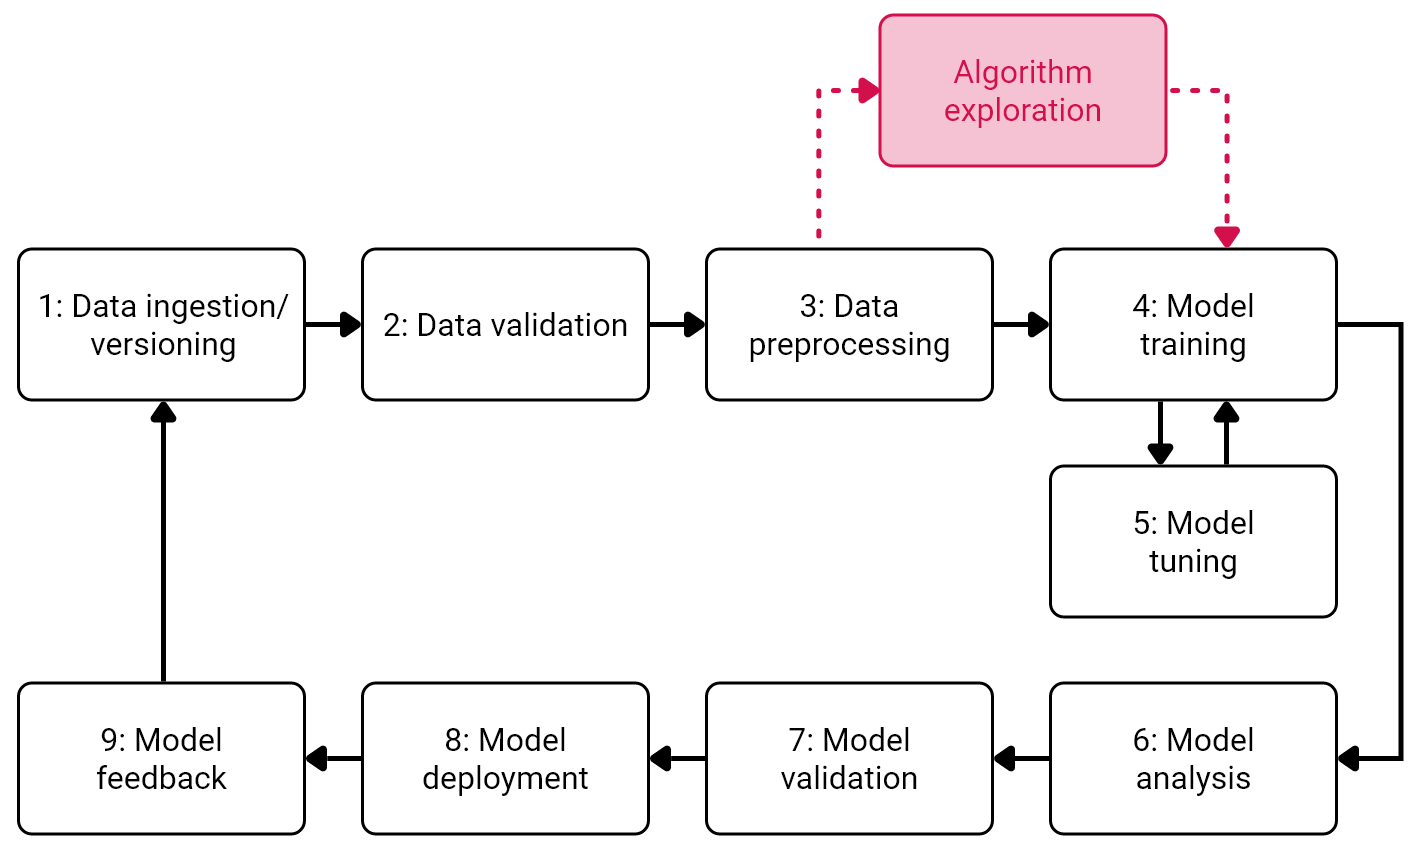
\includegraphics[width=.8\textwidth]{chapter-4/advice-ml-pipeline-lifecycle-v1.png}
  \caption{Machine learning pipeline met een algoritme exploratie tussenstap.}
  \label{fig:advice-ml-pipeline-lifecycle-v1}
\end{figure}

In de "Algorithm exploration"\space stap kunnen verschillende algoritmes dat hetzelfde doel bereiken en een variatie van hyperparameters voor elk algoritme getest worden tegen het dataset. Uit deze tests kan een prestatiescore gegenereerd worden om vervolgens te kiezen voor het algoritme dat het geschiktst lijkt. Na de keuze kan de pipeline verder gaan met de volgende stappen.

\subsection{Machine learning versimpelen}\label{subsec:machine-learning-versimpelen}
Een van de focuspunten is om te onderzoeken in hoeverre ML te vergemakkelijken is voor developers. Met de huidige pipeline is er vrij veel kennis vereist over ML om ermee te werken. Toch kan een groot deel van de stappen geautomatiseerd worden. Tussen elke stap kan een validatie plaatsvinden met een aantal randvoorwaardes waaraan voldaan moeten worden om door te gaan naar de volgende stap. In \autoref{fig:advice-ml-pipeline-lifecycle-v3} is te zien hoe tussen elke stap een validatie plaats vindt. Om bijvoorbeeld van stap 6 (Model analysis) naar stap 7 (Model validation) te gaan, moet het model even goed of zelfs beter presteren dan de voorganger. Hoe veel beter het model moet kunnen presteren is aan een developer. Mocht het zo zijn dat het model niet voldoet, kan de pipeline stopgezet worden.

\begin{figure}[hbt!]
  \centering
  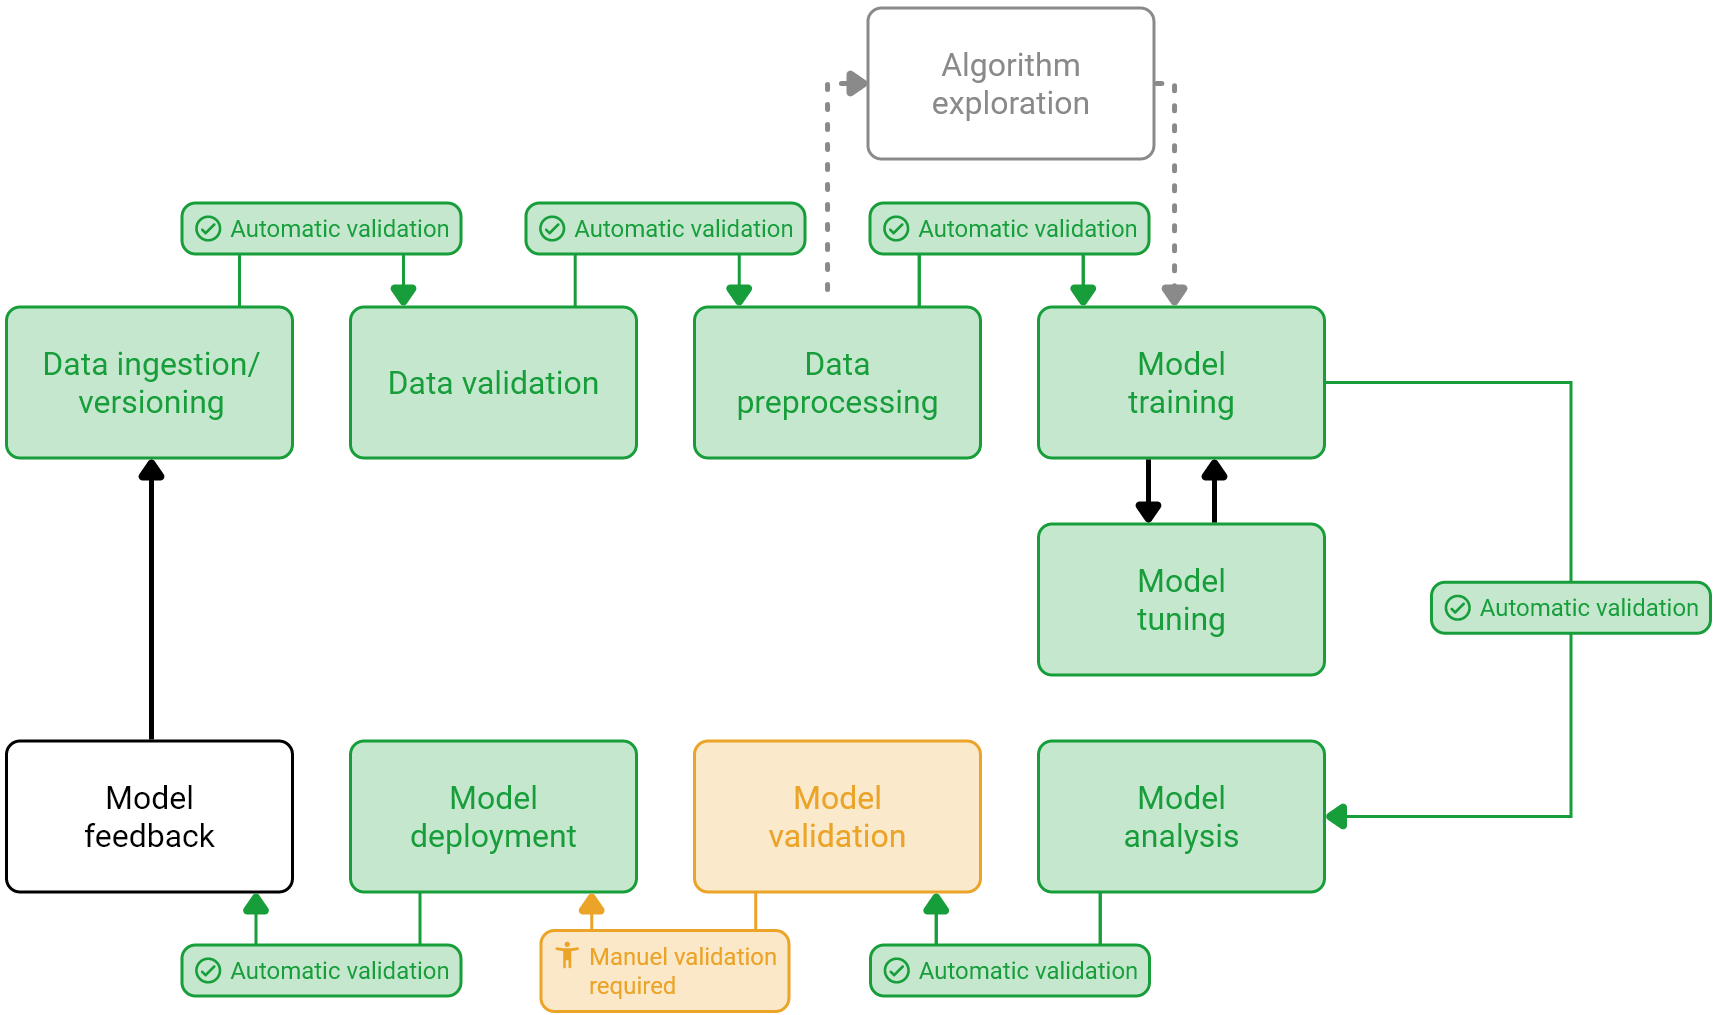
\includegraphics[width=.9\textwidth]{chapter-4/advice-ml-pipeline-lifecycle-v3.png}
  \caption{Machine learning pipeline waarbij stappen geautomatiseerd kunnen worden voor het gemak van developers.}
  \label{fig:advice-ml-pipeline-lifecycle-v3}
\end{figure}

Niet alle aspecten van de pipeline kunnen versimpelt worden. Een van de stappen dat niet kan is stap 7 (Model validation) in \autoref{fig:advice-ml-pipeline-lifecycle-v3}. Deze stap vereist input van een mens aangezien de bias van het model wordt beoordeelt. Wel kunnen rapporten over de bias gegenereerd worden zodat de workflow van developers gestroomlijnd wordt.